\documentclass[tikz,border=2pt]{standalone}
\usepackage{amsmath,amssymb}
\usepackage{tikz}

\begin{document}
% Conditioning on B shrinks the world to B: P(A | B) is the share of B that is also in A.
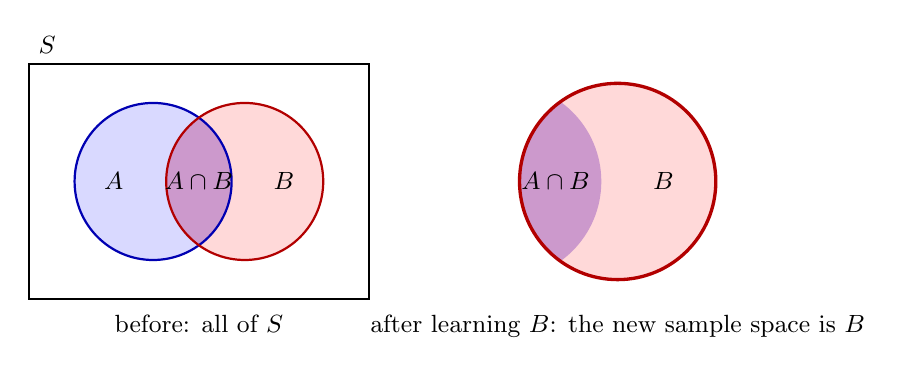
\begin{tikzpicture}[scale=0.831,   every node/.style={font=\small}]
	\begin{scope}
		\draw[thick] (-2.6,-1.8) rectangle (2.6,1.8);
		\node[anchor=south west] at (-2.6,1.8) {$S$};
		\fill[blue!15] (-0.7,0) circle (1.2);
		\fill[red!15] (0.7,0) circle (1.2);
		\begin{scope}
			\clip (-0.7,0) circle (1.2);
			\fill[violet!40] (0.7,0) circle (1.2);
		\end{scope}
		\draw[thick, blue!70!black] (-0.7,0) circle (1.2);
		\draw[thick, red!70!black] (0.7,0) circle (1.2);
		\node at (-1.3,0) {$A$};
		\node at (1.3,0) {$B$};
		\node[font=\small] at (0,0) {$A\cap B$};
		\node[anchor=north] at (0,-1.9) {before: all of $S$};
	\end{scope}
	\begin{scope}[xshift=6.4cm]
		\fill[red!15] (0,0) circle (1.5);
		\begin{scope}
			\clip (0,0) circle (1.5);
			\fill[violet!40] (-1.75,0) circle (1.5);
		\end{scope}
		\draw[very thick, red!70!black] (0,0) circle (1.5);
		\node at (0.7,0) {$B$};
		\node[font=\small] at (-0.95,0) {$A\cap B$};
		\node[anchor=north] at (0,-1.9) {after learning $B$: the new sample space is $B$};
	\end{scope}
	
\end{tikzpicture}
\end{document}
